\documentclass[11pt]{article}

\usepackage[utf8]{inputenc}
\usepackage[T1]{fontenc}

\usepackage[dvipsnames]{xcolor}
\usepackage{blindtext,tcolorbox,graphicx,color}
\usepackage{amssymb,amsmath,amsthm,mathtools,mathabx,hyperref,txfonts,siunitx,booktabs,fontspec}

%Beispiel für farbige boxen:

%\begin{tcolorbox}[width=\textwidth,colback={green},title={With rounded corners},colbacktitle=yellow,coltitle=blue]    
%	\blindtext[1]
%\end{tcolorbox}    
%
%\begin{tcolorbox}[width=\textwidth,colback={red},title={With true corners},outer arc=0mm,colupper=white]    
%	\blindtext[1]     
%\end{tcolorbox} 

\hypersetup
	{ 
		colorlinks=true,       % false: boxed links; true: colored links
		linkcolor=blue,          % color of internal links (change box color with linkbordercolor)
		citecolor=green,        % color of links to bibliography
		filecolor=magenta,      % color of file links
		urlcolor=cyan,           % color of external links
		linkbordercolor	= {1 0 0},
		citebordercolor	= {0 1 0},	
		urlbordercolor	= {0 1 1}
	}

\newcommand{\definition}{\\ \textbf{Definition:} \hspace{1cm} }

\newcommand*{\QEDA}{\hfill\ensuremath{\blacksquare}}%
\newcommand*{\QEDB}{\hfill\ensuremath{\square}}%
\newcommand*{\ds}[1]{{\displaystyle #1}}
\newcommand*{\bild}{\begin{center} \textbf{BILD fehlt hier noch} \end{center}}
\newcommand*{\erg}[2]{\begin{tcolorbox}[width=\textwidth,colback={Orchid},title={#1},colbacktitle=SkyBlue,coltitle=Black] #2  \end{tcolorbox}}

\newcommand*{\kommentar}[1]{\begin{tcolorbox}[width=\textwidth,colback={Lavender}] #1  \end{tcolorbox} }

\begin{document}
	\title{Experimental Physik II Kapitel 19}
		\author
			{
				author\\
				{\small 	\texttt{email}}
			}
		\date{\today}
	\maketitle
	\tableofcontents
	\setcounter{section}{18} %Hier fängt die Nummerierung an.
	\newpage
	
	\section{Wellen}
	
	\begin{center}
	$ t=t_0 $:
\bild
Räumliche Periodizität

\rule{5cm}{.2pt}

$ \vec{r} = \vec{r}_0 $
\bild
zeitliche Periodizität
\end{center}

Welle: Zeitlich und räumlich periodische Auslenkung einer Zustandsänderung.\\
$ \Rightarrow $ Energie- und Impulstransport \underline{ohne} Materialtransport!\\
\paragraph{Experiment} \hfill \\
Einmalige Störung
\bild
$ \Rightarrow $ Kein periodischer Vorgang!

\paragraph{Experiment: WWW} \hfill \\
Periodische Erregung, Ausbreitung ohne Materialtransport!
\begin{itemize}
	\item punktförmiger Erreger: Kreiswellen
	\item linienförmiger Erreger: Ebene Welle
\end{itemize}
\paragraph{Heutz'sche Dipol} \hfill \\
Emission mit charakteristischer Abschallgeometrie
\paragraph{Verdichtungswelle ($ \Rightarrow $ "Wellenmaschine")} \hfill \\
$ \Rightarrow $ Unterschied: \underline{Transversalwelle}, \underline{Longitudinalwelle}

	\subsection{2 Arten von Wellenausbreitung}
\begin{itemize}
	\item Transversalwellen (Transversal Polarisiert) \\
	Schwingungsrichtung $ \perp $ Ausbreitungsrichtung\\
	z.B. Seilwelle:
	\bild
	\begin{center}
		
		2 Möglichkeitden der Polarisierung:
		\bild
		Transversalwellen sind polarisierbar
	\end{center}
	\item Longitudinalwellen (longitudinal Polarisiert)\\
	z.B. Schallwellen
	\bild
\end{itemize}

\underline{Mathematische Beschreibung der Wellenausbreitung}\break \\
"Störung" wandert mit Ausbreitungsgeschwindigkeit $ v_{Ph} $
\bild
\bild
Für mit-bewegten Beobachter bleibt Störung ortsfest (in \emph{S'})
$$ f(x')=f(x-v_{Ph}\cdot t) $$
$ \Rightarrow $ 1-dim Welle kann man beschreiben durch, $ \Psi(x,t) = \underline{\underline{f(x-v_{Ph} \cdot t)}} $ Jeder Punkt der Störung wandert mit $ v_{Ph} $ nach rechts. $$ v_{Ph} \text{: Phasengeschwindigkeit} $$
(Ausbreitung der Störung ohne Verformung!)\\
$ \Phi(x,t) $: Auslenkung, Druck, Dichte, $ \vec{E} $,$ \vec{B} $-Feld Amplitude, ...\\ \break
Sonderfall: Harmonische Wellen
\begin{align*}
\Psi(x,t) &= \Psi_0 \cdot \overbrace{\sin(K\cdot x -\omega t)}^{f(x,t)}\\
& \varphi = K \cdot x = \omega t \text{ : Phase}\\
K&: \text{Wellenzahl}\\
\omega&: \text{Kreisfrequenz}
\end{align*}
\hfill\\
\hypertarget{a}{(a)} \bild
\hypertarget{b}{(b)} \bild
\hyperlink{a}{(a)}
\begin{align*}
\Psi(x,t) = \Psi &= \Psi_0 \cdot \sin(Kx-\omega t)\\
&= \Psi_0 \cdot \sin(K(x+\lambda)-\omega t)\\
&= \Psi_0 \cdot \sin((Kx-\omega t)+K\cdot \lambda)\\
&\Rightarrow K \cdot \lambda = 2\pi &&\lambda \text{:Wellenlänge}\\
&\hspace{5mm} \Rightarrow K = \frac{2\pi}{\lambda}
\end{align*}
\hyperlink{a}{(a)}
\begin{align*}
\Psi &= \Psi_0 \cdot (Kx-\omega t)\\
&= \Psi_0 \cdot \sin(Kx-\omega (t+T))\\
&\Rightarrow\omega \cdot T = 2\pi \Rightarrow \omega = \frac{2\pi}{T} && \underline{T\text{: Periodendauer}}
\end{align*}

Wellen darstellbar:
\begin{align*}
\Psi(x,t) &= \Psi_0 \cdot \sin(Kx-\omega t)\\
&= \underline{\Psi_0 \cdot \sin (2\pi(\frac{x}{\lambda} - \frac{t}{T}))}
\end{align*}
In der Zeit \emph{T} (Periodendauer) breitet sich die Welle um eine Wellenlänge ($ \lambda $) aus.

$$ \Rightarrow \text{ Ausbreitungsgeschwindigketi } \boxed{ v_{Ph} = c = \frac{\lambda}{T} = \lambda \cdot \underset{\text{Frequenz}}{\nu} } $$

\begin{align*}
\Psi^{\pm}(x,t)&=\Psi_0 \cdot \sin(Kx\pm\omega t)\\
\Psi^{+} &\text{: läuft im Ortsraum nach links}\\
\Psi^{-} &\text{: läuft im Ortsraum nach rechts}
\end{align*}
	\subsection{Die Wellengleichung}

Erinnerung: Schwingungsgleichung: $ \ddot{\Psi} + \omega^2 \cdot \Psi = 0 $ \\
Lösung: Harmonische Schwingung: $  \Psi = \Psi_0 \cdot \sin(\omega t) $ \\
Wellen: Periodisch /bisher: auch harmonisch) in Ort und Zeit \\
\indent $ \Rightarrow $  Vermutung: Wellengleichung muss 2. Ableitung enthalten\\
Ansatz für $ \Psi $: $ \Psi(x,t) = \Psi_0 \cdot f(Kx-\omega t) $\\
$ f $ ist beliebig (aber periodische) Funktion der Phase $ \varphi $\\
$$ \frac{\partial\varphi}{\partial x} = K \hspace{5mm};\hspace{5mm} \frac{\partial\varphi}{\partial t} = -\omega$$
2. Ableitung berechnen:\\
Ort:
\begin{align*}
\frac{\partial\Psi}{\partial x} &= \Psi_0 \cdot \frac{\partial f}{\partial \varphi} \cdot \frac{\partial\varphi}{\partial x} && \text{(Kettenregel)} \\
&= \Psi_0 \cdot K \cdot \frac{\partial f}{\partial \varphi} \\
\hfill \\
\frac{\partial^2 \Psi}{\partial x^2} &= \Psi_0 \cdot K \cdot \frac{\partial^2 f}{\partial \varphi^2} \cdot \frac{\partial\varphi}{\partial x} = \Psi_0 \cdot K^2 \cdot \frac{\partial^2 f}{\partial \varphi^2}\\
&\Leftrightarrow {\color{CadetBlue}\underline{\Psi_0 \cdot \frac{\partial^2 f}{\partial \varphi^2} = K^{-2} \cdot \frac{\partial^2\Psi}{\partial x^2}}}
\end{align*}
Zeit:
\begin{align*}
\frac{\partial\Psi}{\partial t} &= \Psi_0 \cdot \frac{\partial f}{\partial\varphi} \frac{\partial\varphi}{\partial t} = -\omega \cdot \Psi_0 \frac{\partial f}{\partial\varphi}\\
\frac{\partial^2\Phi}{\partial t^2} &= \omega^2\cdot\Psi_0\cdot\frac{\partial^2f}{\partial \varphi^2} \Rightarrow {\color{CadetBlue}\underline{\Psi_0\cdot\frac{\partial^2 f}{\partial \varphi^2} = \omega^{-2} \cdot \frac{\partial^2\Psi}{\partial t^2}}}\\
\hfill \\
\Rightarrow &K^{-2} \cdot \frac{\partial^2\Psi}{\partial x^2} = \omega^{-2} \cdot \frac{\partial^2\Psi}{\partial t^2}\\
&\underline{\underline{\frac{\omega^2}{K^2} \cdot \frac{\partial^2\Psi}{\partial x^2} = \frac{\partial^2\Psi}{\partial t^2}}} &&\text{2. Ableitung nach Ort und Zeit verknüpft!!}
\end{align*}

mit $ v_{Ph} = \frac{\omega}{K} \hspace{5mm} \boxed{v^2_{Ph} \cdot \frac{\partial^2\Psi}{\partial x^2} = \frac{\partial^2\Psi}{\partial t^2}} $ ist die Wellengleichung in 1 Dimension! \\

$ f (x-v_{Ph} \cdot t) $ ist Lösung und beschreibt Ausbreitung in positiver x-Richtung!\\
Dann ist auch $ g(x+v_{Ph} \cdot t) $ Lösung, Ausbreitung in negativer x-Richtung!\\
\break
$ \Rightarrow $ Allgemeine Lösung der Wellengleichung:
$$ \Psi(x,t) = f(x-v\cdot t) + g(x+v\cdot t) $$
\begin{center}
	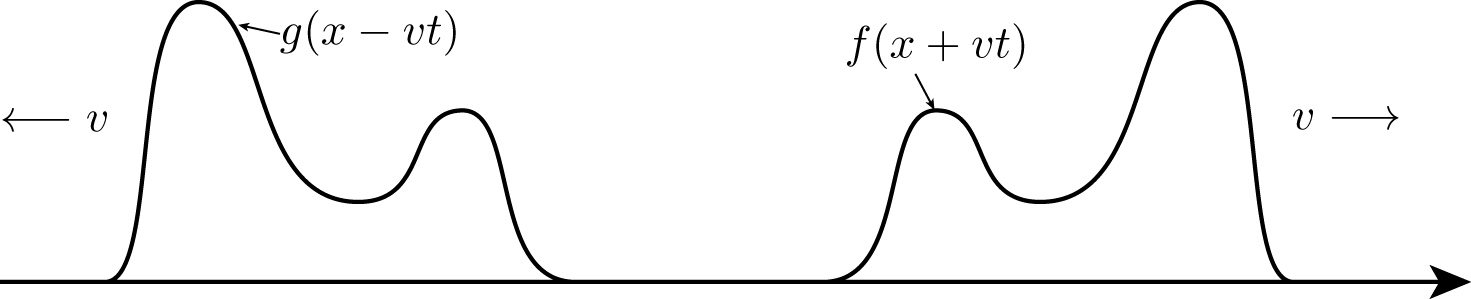
\includegraphics[width=0.7\linewidth]{skizzen/19/19B11}
\end{center}
	\subsection{Überlagerung von Wellen} (in einer Dimension)\\
Superpositionsprinzip: Ungestörte Überlagerung mehrerer Wellen
$$ \Psi(\vec{r},t) = \sum_{i=1}^{N} \Psi_1(\vec{r},t)$$
\underline{Reflexion von Wellen $ \rightarrow $ stehende Wellen}\\
Experiment: Reflexion der Welle einer Pendelkette
\begin{itemize}
	\item Festes Ende: Phasensprung von $ \pi $ bei Reflexion
	\bild
	\item Freies Ende: Kein Phasensprung
	\bild
\end{itemize}
Überlegung von links- und rechts-laufender Welle\\
Gleiche Amplitude, gleiche Frequenz, Phasenverschiebung $ \varphi $
\begin{align*}
\Psi(x,t) &=\Psi_0 \cdot \cos(Kx-\omega t) \pm \Psi \cdot \cos(Kx+\omega t + \varphi)\\
\text{Additionstheroeme} \rightarrow &= \underline{\underline{2\cdot\Psi_0\cdot\cos(\omega t + \frac{\varphi}{2}) \cdot \cos(Kx+\frac{\varphi}{2})  } }
\end{align*}
Faktorisieren der Orts- und Zeitabhängigkeit:\\
Für alle $ t $ gibt es Punkte x; bei denen  $ \Psi(x,t) = 0 $: "Knoten"\\
Betrachte Orts-Teil: Festes Ende: $ \varphi = \pi $\\
Knoten: $ \underbrace{\cos(Kx+\frac{\varphi}{z})}_{\Rightarrow \text{Knoten bei } x_0, x_0+\frac{\pi}{2}, x_0+\frac{3\pi}{2}...} = 0 \Rightarrow Kx+\overbrace{\frac{\varphi}{2}}^{\pi/2}= \frac{(2\mathbb{N}+1)}{2} \cdot \pi $\\ \break
Resonanz-Situation: $  \underset{K=\frac{2\pi}{2}}{K} \cdot x = \frac{(2\mathbb{N}+1)}{2} \cdot \pi $\\
\begin{center}
	Resonanz: $ \underset{\text{Länge}}{L} = \frac{\mathbb{N}}{2} \cdot \lambda $\\
\underline{$ \Rightarrow \lambda = \frac{2}{\mathbb{N}}\cdot L $}\\
\underline{$ \mathbb{N}\cdot\frac{\lambda}{2} = L $}\\
\end{center}
 \bild
 Loses Ende: $ \varphi = 0 $!
 \begin{align*}
 \Rightarrow &\text{ Resonanz: } \frac{2\mathbb{N}+1}{2} \cdot \lambda = L\\
 &\lambda = \frac{4 \cdot L}{(2\mathbb{N}-1)}
 \end{align*}
 \bild
 Mikrowelle:
 \begin{align*}
 d_{Knoten} &= \frac{\lambda}{2} \approx \SI{10}{\centi\meter}\\
 \nu & = \frac{c}{\lambda} = \frac{\SI{3e8}{\meter\per\second}}{\SI{0,2}{\meter}} = \SI{1,5e9}{\per\second}\\
 &=\underline{\SI{1,5}{\giga\hertz}}
 \end{align*}
 \bild
 \bild
 
 \subsubsection{Wellenpakete und Synthese/Analyse nicht harmonischer Wellen} \hfill \\
 Eine streng monochromatische ($ \omega=\omega_0 $, harmonisch) Welle ist zeitlich und räumlich unendlich ausgedehnt! Alle nicht-harmonischen Wellen sind als Überlagerung harmonischer Wellen darstellbar. \\
 Schwingungsanteil: $ \underset{\text{\underline{Fourier-Zerlegung}}}{\boxed{\Psi(t) = a_0 + \sum_{n=1}^{\infty} a_n \cdot \cos(n\cdot\omega_1\cdot t + \varphi_n)}} $ \\
 Auch für Wellenzüge möglich!
 \bild
 \bild
 \bild
 \begin{itemize}
 	\item Darstellung ist immer durch Überlagerung der Grundwelle mit harmonischen Oberwellen möglich.
 	\item Amplituden nehmen mit wachsender Frequenz ab!
 	\item Obertonspektrum ($ a_n $ von $ \omega_n = b\cdot \omega_1 $) ist charakteristisch für den individuellen Klang der Stimme! Es hängt von der Beschaffenheit des "Klangkörpers" ab!
 \end{itemize}
 Überlagerung von Wellen mit ähnlichem $ K,\omega $ bei gleicher Ausbreitungsrichtung und Amplitude.\\
 \rule{5cm}{.2pt}\\
 \bild
 \begin{align*}
 	\Psi(x,t) = \Psi_0 &\left[ \underbrace{\sin(Kx-\omega t) }_{\text{1. Welle}}+ \underbrace{\sin\left( (K+\Delta K)x-(\omega+\Delta\omega)t\right) }_{\text{2. Welle}} \right]\\
 	\sin\alpha+&\sin\beta = 2\cdot\cos\frac{(\alpha-\beta)}{2} \cdot \sin\frac{(\alpha+\beta)}{2}\\
 	\alpha &=(K+\Delta K)x-(\omega+\Delta\omega) \cdot t\\
 	\beta &= Kx-\omega t\\
 	\text{Näherung:}& \frac{\omega + (\omega + \Delta\omega)}{2} \approx \omega \hspace{3mm} ,\hspace{3mm} K+...\\
 	\Psi(x,t) = 2 \Psi_0 & \cdot \underbrace{\cos(\frac{1}{2}(\Delta K \cdot x - \Delta\omega\cdot t) )}_{\text{Modulation der Amplitude}} \cdot \underbrace{\sin(Kx-\omega t)}_{\text{Welle}}
 \end{align*}
 \bild
 \subsubsection{Gruppengeschwindigkeit}
 Wie schnell bewegt sich die cos-Modulation (Einhüllende) im Raum?\\
 Amplitudenfaktor; $ 2 \cdot \Psi_0 \cdot \cos(\frac{1}{2}(\Delta K \cdot x - \Delta\omega \cdot t)) = const.$\\
 (bedenke: feste Phase der Einhüllenden!)\\
 \begin{align*}
 	\Delta K \cdot - \Delta\omega\cdot t &= 0\\
 	\overset{\Delta\omega\rightarrow 0}{\Rightarrow} x &= \frac{d\omega}{dK} \cdot t\\
 	&= v_{Gr} \cdot t
 \end{align*}
 Ausbreitung der Modulation (oder Wellengruppe) mit $ v_{Gr} = \frac{d\omega}{dK} $\\
 $$ \underline{v_{Gr} \text{ Gruppengeschwindigkeit}} $$
 Mit $ v_{Gr} $ breiten sich Informationen (Signale) aus!
 \subsubsection{Phasen- vs Gruppengeschwindigkeit}
 \begin{align*}
 	v_{Gr} = \frac{d\omega}{dK} &= \frac{d}{dK} (v_{Ph} \cdot K) &&K=\frac{2\pi}{\lambda} \hspace{3mm};\hspace{3mm}\lambda=\frac{2\pi}{K}\\
 	&=v_{Ph} + K \cdot \frac{dv_{Ph}}{dK} &&\frac{d\lambda}{dK} = - \frac{2\pi}{K^2}\\
 	\left( \frac{dv_{Ph}}{dK} = \frac{dv{Ph}}{d\lambda} \cdot \frac{d\lambda}{dK}  \right) \\
 	v_{Gr} &= v_{Ph} -  \frac{2\pi}{K} \cdot \frac{ dv_{Ph} }{d\lambda} \\
 	&\boxed{v_{Gr} = v_{Ph} - \lambda \cdot \frac{ dv_{Ph} }{d\lambda} }
 \end{align*}
 $ v_{Gr}  = v _{Ph} $ wenn $ v_{Ph} $ unabhängig von $ k $ , $ \lambda $\\
 wenn $ v_{Ph} \neq v_{Ph}(\lambda) $ : Alle Fourier-Komponenten breiten sich mit gleicher Geschwindigkeit aus! Dann heißt die Welle "dispersionsfrei"!\\
 Sonst: $ v_{Gr} \neq v_{Ph} $ , dann: Wellenpaket läuft auseinander! \underline{($ \Rightarrow $ Dispersion)}\\
 \hfill \\
 Experiment: Wasserwellen sind dispersionsfrei!
 \bild
 Beispiele\\
 Seilwellen
 \bild
 Seil erfährt Spannung: $ \underset{\text{Seilspannung}}{\tau} = \frac{\overset{\text{Kraft}}{F_0}}{\underset{\varnothing \text{-Fläche}}{A}} $\\
 Auslenkung in \emph{y}-Richtung: Rückstellkraft\\
 Wellen in \emph{x}-Richtung: Transversalwelle\\
 \begin{align*}
 	F_2 &= \tau\cdot A \cdot\sin\alpha_2 &&\alpha_1>\alpha_2\\
 	F_1 &= \tau\cdot A \cdot\sin\alpha_1
 \end{align*}
 Wenn betrachtetes Element klein ist, dann:
 \begin{align*}
 	F_y &= F_1 - F_2 \hspace{5mm} \text{(nach einsetzen!)}\\
 	&= \tau \cdot A \cdot (\sin\alpha_1 - \sin\alpha_2)\\
 	&\approx\tau \cdot A \cdot ( \alpha_1 - \alpha_2) = \tau \cdot A \cdot \Delta\alpha
 \end{align*}
 $ \Rightarrow \Delta M $ wird beschleunigt: $  \Delta M = \Delta x \cdot A \cdot \underset{Massendichte}{\rho} $  (im GG)\\
 \begin{math}
 	F_y = \Delta M \cdot \frac{d^2y}{dt^2} = \rho \cdot \cancel{A} \cdot \Delta x \cdot \frac{d^2y}{dt^2} = \tau \cdot \cancel{A} \cdot \Delta\alpha\\
 	\Leftrightarrow \tau\cdot\frac{\Delta\alpha}{\Delta x} = \rho \cdot \frac{d^2y}{dt^2}\\
 	\alpha = \frac{dy}{dx} \Rightarrow \frac{d\alpha}{dx} = \frac{d^2y}{dx^2} \hspace{5mm} \text{für } \Delta x \rightarrow 0\\
 	\Rightarrow \tau \cdot \frac{d^2y}{dx^2} = \rho \cdot \frac{d^2y}{dt^2}\\
 	\text{Wellengleichung } \boxed{\frac{\tau}{\rho} \cdot \frac{d^2y}{dx^2} = \frac{d^2y}{dt^2} }\\
 	v^2_{Ph} \cdot \frac{d^2\Psi}{dx^2} = \frac{d^2\Psi}{dt^2}\\
 	\Rightarrow v_{Ph} = \underline{\sqrt{\frac{\tau}{\rho}}} = \sqrt{\frac{\tau \cdot A}{\rho \cdot A}} = \sqrt{\frac{F}{\underset{\text{lineare Massendichte}}{\mu}}}\\
 	v_{Ph} = \frac{\omega}{K} \Rightarrow \omega = \sqrt{\frac{\tau}{\rho}} \cdot K\\
 \end{math}
 \bild
 \underline{Keine Dispersion!}\\
 \hfill \\
 Beidseitig eingespannte Seite
 \bild
 Lösung der Wellengleichung: Stehende Welle\\
 \begin{align*}
 	\Psi = \Psi_0 & \cdot \sin Kx \cdot \cos \omega t\\
 	\underset{\text{Knoten}}{\Psi = 0} \text{ :} \hspace{5mm} y=0\hspace{2mm};\hspace{2mm}&\underset{\text{2. RB}}{x=L} \text{ für alle } t\\
 	\Rightarrow K \cdot L = &n \cdot \pi\\
 	\Rightarrow \underline{\underline{\lambda_n = \frac{2}{n} \cdot L}}
 \end{align*}
 Dies definiert die Schwingungsmoden der Seite\\
 $$ 2\pi\nu_n $$
 Dispersion: $ \omega_n = \sqrt{\frac{\tau}{\rho}} \cdot K_n = = \sqrt{\frac{\tau}{\rho}} \cdot \frac{2\pi}{\lambda_n} $
 $$ \Rightarrow \underline{\underline{\nu_n = \sqrt{\frac{\tau}{\rho}} \cdot \lambda_n^{-1} = \frac{n}{2L} \cdot \sqrt{\frac{\tau}{\rho} } } } $$
 Saiteninstrument:
 \begin{itemize}
 	\item $ \lambda $ durch Geometrie bestimmt
 	\item zugehörige Frequenz durch Spannung eingestellt!
 \end{itemize}
 $ \Rightarrow $ Umwandlung von stehender Welle in Schallwelle\\
 Klang: Obertöne gleichzeitig angeregt; Superposition von Grund- und Oberschwingung
 $$ \Psi(x,t) = \sum_{i=1}^{\infty} \Psi_{0,n} \sin(K_nx) \cdot \cos(\omega_nt) $$
 $$ \Rightarrow \underline{v_S = \frac{d\omega}{dK} = \sqrt{\frac{\tau}{\rho}} = v_{Ph}} $$
\end{document}
